% \documentstyle[a4paper,twocolumn,11pt]{jarticle}
\documentclass[a4paper,twocolumn,11pt]{jarticle}

%
%\setlength{\oddsidemargin}{-7 mm}
%\setlength{\evensidemargin}{0 mm}
%\setlength{\topmargin}{-17 mm}
%\setlength{\textheight}{240 mm}
%\setlength{\textwidth}{170 mm}
%\setlength{\columnsep}{1.5em}
\setlength{\oddsidemargin}{-12 mm}
\setlength{\evensidemargin}{0 mm}
\setlength{\topmargin}{-27 mm}
\setlength{\textheight}{275 mm}
\setlength{\textwidth}{185 mm}
\setlength{\columnsep}{1.5em}
\newcommand{\qed}{\hspace*{\fill} $\Box$ }
%
\makeatletter
\renewcommand{\@maketitle}{%
  \newpage
  \null
  \begin{center}%
  \let \footnote \thanks
    {\LARGE \bf \@title \par}%
    \vskip 10pt
    {\normalsize \@author \par}%
    \vskip 5pt
  \end{center}%
  \par
  \vskip 0.5em 
}
\renewcommand{\section}{\@startsection {section}{1}{\z@}%
{4.0pt plus 6.0pt minus 3.0pt}%
{2.0pt plus 2.0pt minus 2.0pt}{\large\bf }}
\renewcommand{\subsection}{\@startsection{subsection}{2}{\z@}%
{4.0pt plus 4.0pt minus 3.0pt}%
{1.0pt plus 2.0pt minus 1.0pt}{\large\bf }}
\renewcommand{\subsubsection}{\@startsection{subsubsection}{3}{\z@}%
{4.0pt plus 4.0pt minus 3.0pt}%
{1.0pt plus 2.0pt minus 1.0pt}{\large\bf }}
\renewcommand{\paragraph}{\@startsection{paragraph}{4}{\z@}%
{0.0pt plus 1.0pt minus 0.0pt}{2.0pt plus 1.0pt}%
{\normalsize\bf}}
\renewcommand{\subparagraph}{\@startsection{subparagraph}{4}%
{\parindent}{0.0pt plus 1.0pt minus 0.0pt}{2.0pt plus
1.0pt}{\normalsize\bf}}
\renewcommand{\thesection}{\arabic{section}.}
\renewcommand{\thesubsection}{\arabic{section}.\arabic{subsection}.}
\renewcommand{\thesubsubsection}{\arabic{section}.\arabic{subsection}.\arabic{subsubsection}}
\makeatother

\usepackage[dvipdfmx]{graphicx}
% \usepackage{amsmath,amsfonts}
\usepackage{bm}
%

\title{電子教材の閲覧データとコンテンツ情報を用いた学習者のスコア予測}


\author{JB19S029 小岸沙也加 
\\ 指導教員:川嶋宏彰教授}
%
\date{2023/02/02}
%
%
%↓索引生成
%\makeindex
%

\begin{document}
\maketitle
\newtheorem{thm}{定理}
\newtheorem{df}[thm]{定義}
\newtheorem{lm}[thm]{補題}
\newtheorem{co}[thm]{系}
\newtheorem{pr}[thm]{命題}
\newtheorem{que}[thm]{問題}

\thispagestyle{empty}

\section{序論}

% なげえ

講義で使用される資料の閲覧に,デジタル教材の配信システム上に教師がアップロードした講義資料をオンラインで閲覧する形態が用いられるようになっている.このようなシステムが使用されることにより,詳細な操作ログを取得できる.
この閲覧データを解析することで各学生の理解度や,つまずき箇所を推定できれば,個々の学生に早い段階でアプローチすることができ,学生の学力向上に繋がると期待できる.
% 学生の行動から成績予測を行った研究として,デジタル教材の配信システムのひとつである BookRoll システムから得た閲覧データを用いて,毎週の生徒の成績を予測し,
% 受講期間中に随時リスクのある学生とない学生に分類する試み~\cite{Predictionstudentperformance2022}や,
% ニューラルネットワークの解釈手法を用いて
% どのような学習行動が成績に関連するかを調べた研究~\cite{BR12020}がある.
学生の閲覧データを使用した先行研究
% ~\cite{Predictionstudentperformance2022, BR12020}
% は多くされている一方で,
はあるが,学生が講義で使用する講義資料そのものの情報を成績予測に用いることの有効性については十分検証されていない.

そこで本研究では,閲覧データに加えて,講義で使用された資料(本稿では「コンテンツ」と呼ぶ)のテキスト情報を利用することで,各学生の理解度の推定精度向上を目指す.
ここで理解度とは,毎週講義後に行われる小テストの点数(スコア)とし,閲覧データはBookRollシステムで得られた操作ログを用いる.このとき,コンテンツ情報の利用が小テストのスコア予測にどれだけ貢献するかを検証する.

\noindent{\bf BookRollシステム}\quad 
BookRollシステム~\cite{BookRoll}は,教員がアップロードした講義資料や教材を学生がオンライン上で閲覧できるシステムである.
閲覧データとしては,たとえばコンテンツを開く/閉じる,ページを移動する,
% 次のページへ進む,一つ前のページへ戻る,
マーカーやメモを付与する,コンテンツ内検索を行うといった操作を行ったタイミングで,その操作タイプが,操作を行った学生のID,日時,コンテンツ番号,ページ番号などの情報と共に記録される.

\section{コンテンツを利用したスコア予測}\label{sec:scoreprediction}
% \subsection{学習者のスコア予測}

図~\ref{fig:overview}は本研究の全体像である.
本研究では学生の行動からスコア予測を行うベースラインに加えて,
% 実際に使用されたコンテンツの情報を含めて学習者のスコア予測を行う.
% 予測手法として,
% 本研究では学生の行動からのスコア予測をベースラインとして,
学生が長く閲覧したコンテンツに含まれるテキスト情報を用いる手法
% 1と小テストに関係するページの情報を使用する手法2
を提案する.
% 閲覧データは2020年に九州大学で7週間行われた講義のデータを使用する.
% 予測には,
2020年に九州大学で7週間100名の学生に対し行われた,情報系科目の講義の
% BookRollシステムの
閲覧データおよび
% 講義で用いられた
コンテンツを用いて,講義中に行われた小テストの結果(小テストデータ)をLightGBMで予測する.

閲覧データより,各学生について,あるコンテンツの各ページにおける操作タイプごとの操作回数および閲覧時間を求め,これら特徴量を要素とするようなベクトルを各学生の「行動特徴ベクトル」と呼ぶ.
ここで,学生$i$のコンテンツ$c$における行動特徴ベクトルを$\bm{u}^{(i)}_c$と表す.ページの情報のベクトル化には,事前学習済みのSentence-BERT~\cite{sonoisa}を使用し,ページベクトル$\bm{v}_{(c,p)}$とする.
% $\bm{u}^{(i)}_c$の次元数は「ページ数 $\times$ (操作タイプ数 + 1)」(最後の1は閲覧時間に対応)であり,ページ数はコンテンツ$c$によりそれぞれ異なる..
% 手法1では,
さらに,学生$i$がコンテンツ$c$において長く閲覧したページの内容情報を多く含む「閲覧コンテンツベクトル」$\bm{v}^{(i)}_c$を学生$i$のページ$p$に対する閲覧時間の総和$t^{(i)}_{(c,p)}$に基づいてページベクトルに重みづけを行って足し合わせることで求める.
ただし,継続して5分より長く同じページを閲覧されたログは放置されたものとして除く.
この閲覧コンテンツベクトル$\bm{v}^{(i)}_c$を
行動特徴ベクトル$\bm{u}^{(i)}_c$に連結し,
% この統合された特徴ベクトルを用いて,
小テストのスコア予測を行う.
% 方法を提案する.
% ページベクトル$\bm{v}_{(c,p)}$に閲覧時間をかけ,線形和をとる.

% 手法2では,小テストの問題文,解答の選択肢をベクトル化し,ページベクトルとの類似度を求め類似度0.4以上を重みとし,対応するページの行動特徴ベクトル$\bm{u}^{(i)}_c$に重みづけを行ったベクトルで予測を行う.
% ベースラインとして,
閲覧コンテンツベクトル$\bm{v}^{(i)}_c$のみを使用した場合でもスコア予測を行い,予測精度を比較する.

% \subsection{行動特徴ベクトルとコンテンツ情報を用いたスコア予測 (手法1) }

% \subsection{小テストに関係するページを使用したスコア予測 (手法2) }
% さらっとながそう
% でも軽く結果はかくよ
% でも結果書くと2枚にわたらない?

\begin{figure}[tbp]
  \centering
  \vspace{-8mm}
  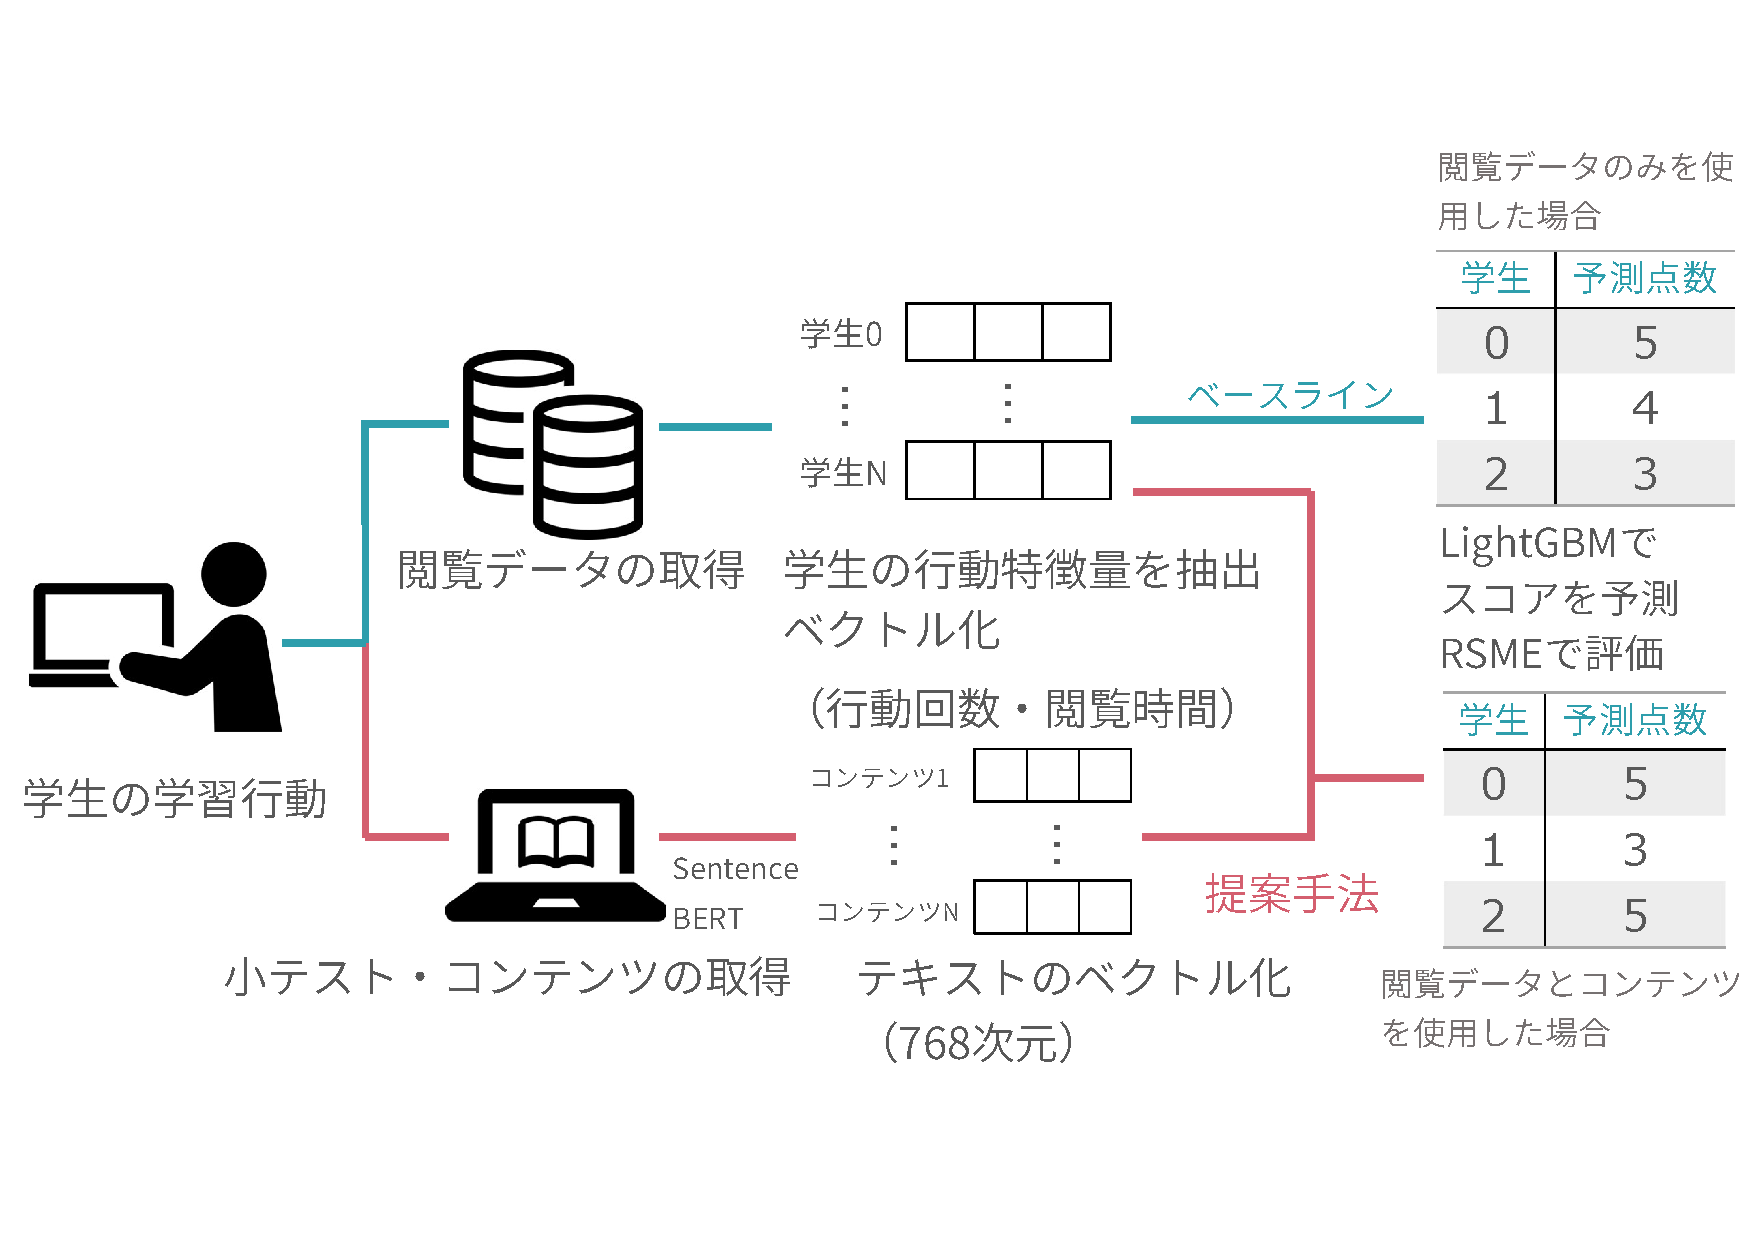
\includegraphics[width=0.9\linewidth]{zentaizo2n.pdf}
  \vspace{-10mm}
  \caption{本研究の全体像}
  \label{fig:overview}
  \vspace{-8mm}
\end{figure}

\section{結果および結論}

図~\ref{fig:rmse_2}にベースライン,閲覧コンテンツベクトルのみで予測,提案手法1,それぞれ5-foldのCVでRMSEを計算した結果を示した.予測は小テストごとに求めているため,平均を示している.
図より,講義時間外含む場合でも,講義時間および前後1時間に行動を絞った場合でも提案手法1がRMSEの平均の値が小さく,予測精度がよかった.
% が最も良い結果となった.
結果より,
% 学生の行動の情報にコンテンツ情報を加えてスコア予測を行うことは有効であると考える.
学生の行動情報と共にコンテンツ情報を用いることは有効であるといえる.

\begin{figure}[tbp]
  \centering
  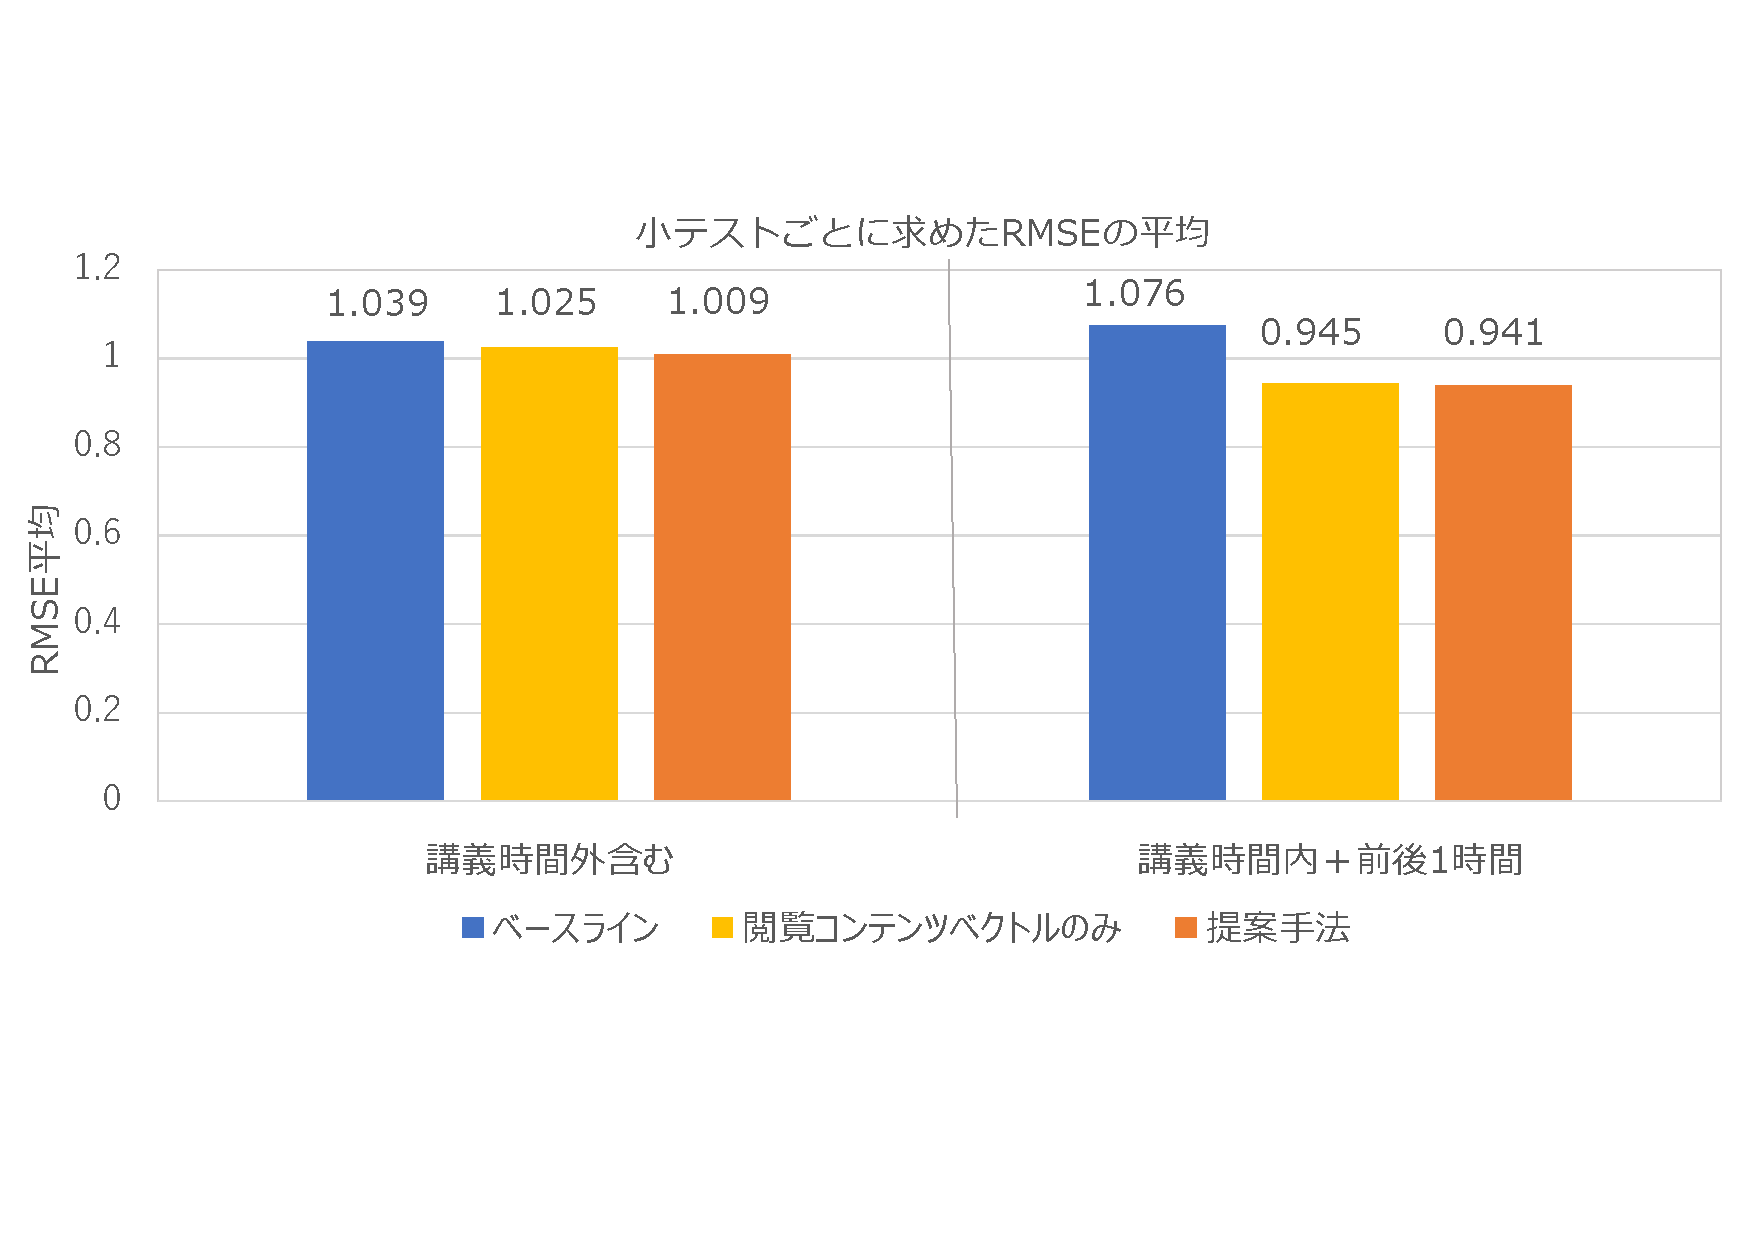
\includegraphics[width=0.9\linewidth]{RMSE_5s.pdf}
  \vspace{-16mm}
  \caption{小テストごとに求めたRMSEの平均}
  \label{fig:rmse_2}
  \vspace{-2mm}
\end{figure}



\fontsize{9pt}{9pt}\selectfont
\bibliography{sotsuronkogishi}
\bibliographystyle{junsrt}



\end{document}
